% Préambule commun des schémas TikZ (compilés séparément par construire_figures.py)
\documentclass[tikz,border=3pt]{standalone}
\usepackage[T1]{fontenc}
\usepackage[utf8]{inputenc}
\usepackage{lmodern}
\usepackage{amsmath,amssymb}
\usepackage{bm}
\usepackage[american,siunitx,straightvoltages]{circuitikz}
\usetikzlibrary{arrows.meta,positioning,calc,decorations.pathmorphing,
  decorations.markings,decorations.pathreplacing,patterns,shapes.geometric,
  shapes.misc,shapes.multipart,fit,backgrounds,3d,intersections,matrix}

\ctikzset{bipoles/length=1.1cm, amplifiers/scale=0.85, tripoles/op amp/width=1.4}

\tikzset{
  >={Latex[length=2mm,width=1.4mm]},
  every picture/.style={line width=0.6pt, font=\small},
  % schémas-blocs
  bloc/.style={draw, minimum width=1.5cm, minimum height=0.9cm, align=center,
               inner sep=3pt, fill=white},
  somme/.style={draw, circle, minimum size=4.5mm, inner sep=0pt, fill=white,
                path picture={\draw (path picture bounding box.north west)
                  -- (path picture bounding box.south east)
                  (path picture bounding box.north east)
                  -- (path picture bounding box.south west);}},
  gain/.style={draw, isosceles triangle, isosceles triangle apex angle=60,
               minimum size=8mm, inner sep=1pt, fill=white},
  bruit/.style={draw, circle, minimum size=4.5mm, inner sep=0pt, fill=white,
                path picture={\node at (path picture bounding box.center)
                  {\scriptsize$\ast$};}},
  cadre/.style={draw, dashed, rounded corners=1pt},
  cadrept/.style={draw, dash dot, rounded corners=1pt},
  fleche/.style={->},
  % mécanique
  bati/.style={pattern=north east lines, draw=none},
  ressort/.style={decorate, decoration={coil, aspect=0.4, segment length=2.2mm,
                  amplitude=2mm, pre length=2mm, post length=2mm}},
  zigzag/.style={decorate, decoration={zigzag, segment length=2mm,
                  amplitude=1.6mm, pre length=2mm, post length=2mm}},
  pivot/.style={draw, circle, fill=white, minimum size=2.2mm, inner sep=0pt},
  masse/.style={draw, fill=gray!25, minimum width=1.4cm, minimum height=0.8cm},
  cote/.style={<->, line width=0.4pt},
  axe/.style={->, line width=0.6pt},
  trait mixte/.style={dash dot, line width=0.4pt},
}

% Encastrement / bâti hachuré : \bati{(x1,y1)}{(x2,y2)} trace une ligne et ses hachures dessous
\newcommand{\bati}[3][0.18]{%
  \fill[pattern=north east lines] #2 rectangle ($#3+(0,-#1)$);
  \draw[line width=0.8pt] #2 -- #3;}

% Transducteur (deux cercles entrelacés) : \pic (t) at (x,y) {transducteur};  -> (t-o) entrée, (t-e) sortie
\tikzset{
  transducteur/.pic={\draw (-0.13,0) circle (0.24); \draw (0.13,0) circle (0.24);
    \coordinate (-o) at (-0.37,0); \coordinate (-e) at (0.37,0);
    \coordinate (-n) at (0,0.24); \coordinate (-s) at (0,-0.24);},
  bobine/.style={decorate, decoration={coil, aspect=0.7, segment length=1.4mm,
                 amplitude=1.6mm, pre length=1mm, post length=1mm}},
  sourcebruit/.style={draw, circle, minimum size=5mm, inner sep=0pt, fill=white,
                 label={[inner sep=0pt]center:$\ast$}},
  sourcecourant/.style={draw, circle, minimum size=5mm, inner sep=0pt, fill=white,
                 label={[inner sep=0pt]center:$\circledast$}},
}

% Composants compacts (pour les petits boîtiers des schémas-blocs)
\newcommand{\resistance}[2]{% de #1 à #2 (quelconque)
  \draw #1 -- ($#1!0.22!#2$) ($#1!0.78!#2$) -- #2;
  \draw[decorate, decoration={zigzag, segment length=1.5mm, amplitude=1.1mm}]
    ($#1!0.22!#2$) -- ($#1!0.78!#2$);}
\newcommand{\condensateur}[2]{% horizontal de #1 à #2
  \draw #1 -- ($($#1!0.5!#2$)+(-0.05,0)$) ($($#1!0.5!#2$)+(0.05,0)$) -- #2;
  \draw[line width=1pt] ($($#1!0.5!#2$)+(-0.05,0.14)$) -- ($($#1!0.5!#2$)+(-0.05,-0.14)$)
                        ($($#1!0.5!#2$)+(0.05,0.14)$) -- ($($#1!0.5!#2$)+(0.05,-0.14)$);}
% R // C horizontal : \RparC{(x,y)}{longueur}{écart}  (centre, longueur totale, écart vertical)
\newcommand{\RparC}[3]{%
  \coordinate (rcA) at ($#1+(-#2/2,0)$); \coordinate (rcB) at ($#1+(#2/2,0)$);
  \draw (rcA) -- ++(0.15,0) coordinate (rcA1) (rcB) -- ++(-0.15,0) coordinate (rcB1);
  \draw (rcA1) -- ++(0,#3/2) (rcA1) -- ++(0,-#3/2) (rcB1) -- ++(0,#3/2) (rcB1) -- ++(0,-#3/2);
  \resistance{($(rcA1)+(0,#3/2)$)}{($(rcB1)+(0,#3/2)$)}
  \condensateur{($(rcA1)+(0,-#3/2)$)}{($(rcB1)+(0,-#3/2)$)}}

\begin{document}
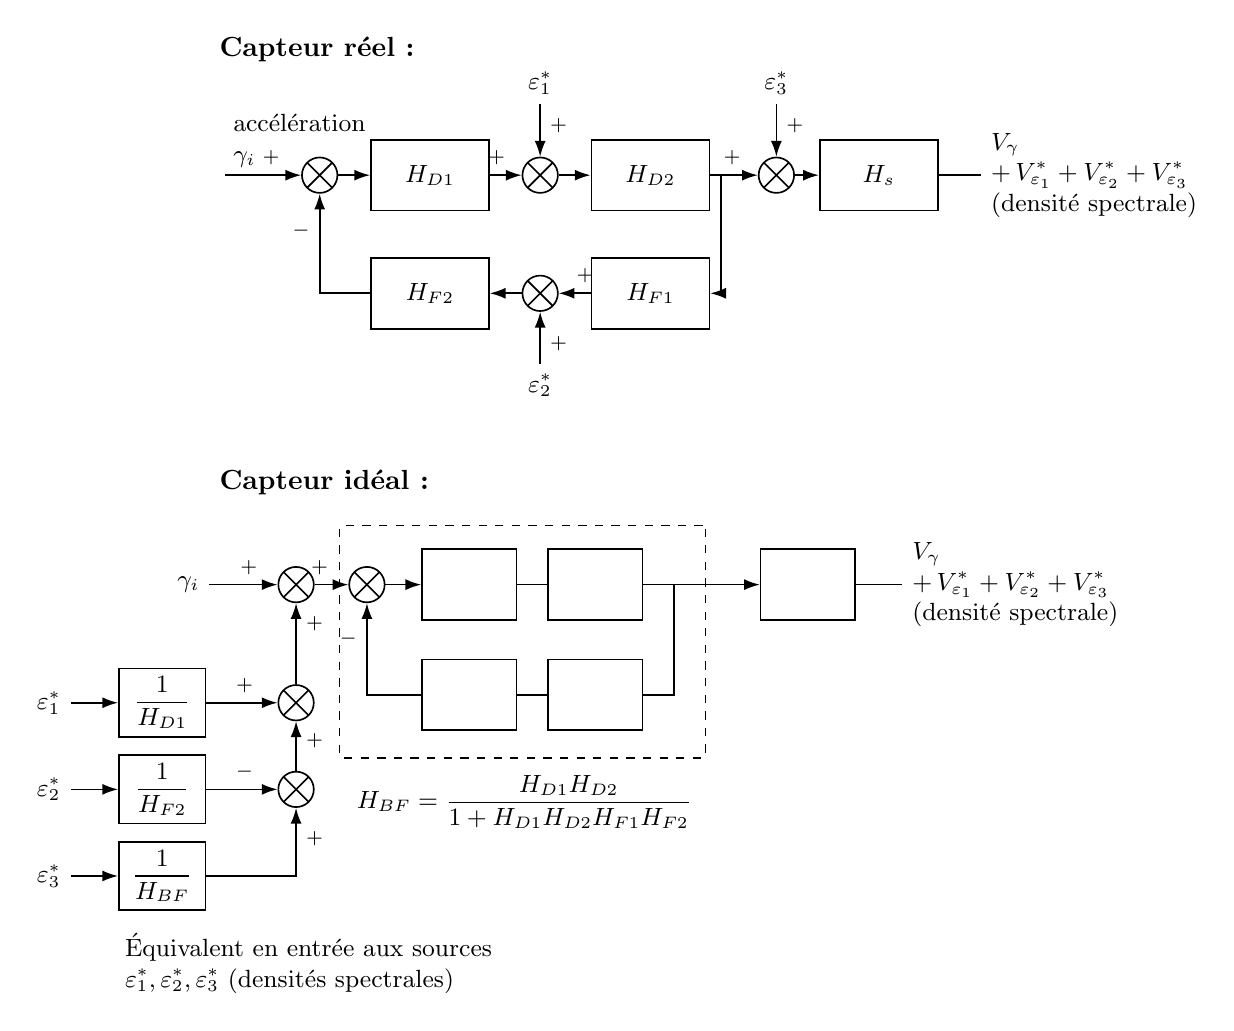
\begin{tikzpicture}[font=\small]
  % ---------- capteur réel ----------
  \node[font=\bfseries, anchor=west] at (-1.4,1.6) {Capteur réel :};
  \node[somme] (s1) at (0,0) {};
  \node[bloc] (d1) at (1.4,0) {$H_{D1}$};
  \node[somme] (s2) at (2.8,0) {};
  \node[bloc] (d2) at (4.2,0) {$H_{D2}$};
  \node[somme] (s3) at (5.8,0) {};
  \node[bloc] (hs) at (7.1,0) {$H_s$};
  \node[bloc] (f2) at (1.4,-1.5) {$H_{F2}$};
  \node[somme] (s4) at (2.8,-1.5) {};
  \node[bloc] (f1) at (4.2,-1.5) {$H_{F1}$};
  \draw[->] (-1.2,0) node[above right=-1pt, align=left] {accélération\\$\gamma_i$} -- (s1) node[above left, pos=0.85] {\scriptsize$+$};
  \draw[->] (s1) -- (d1); \draw[->] (d1) -- (s2) node[above left, pos=0.8] {\scriptsize$+$};
  \draw[->] (s2) -- (d2); \draw[->] (d2) -- (s3) node[above left, pos=0.85] {\scriptsize$+$};
  \draw[->] (s3) -- (hs);
  \draw (hs.east) -- (8.4,0) node[right, align=left] {$V_\gamma$\\$+\,V_{\varepsilon_1}^* + V_{\varepsilon_2}^* + V_{\varepsilon_3}^*$\\(densité spectrale)};
  \draw[->] (5.1,0) |- (f1.east); \draw[->] (f1) -- (s4) node[above right, pos=0.75] {\scriptsize$+$};
  \draw[->] (s4) -- (f2); \draw[->] (f2.west) -| (s1.south) node[below left, pos=0.9] {\scriptsize$-$};
  \draw[->] (2.8,0.9) node[above] {$\varepsilon_1^*$} -- (s2) node[right, pos=0.4] {\scriptsize$+$};
  \draw[->] (5.8,0.9) node[above] {$\varepsilon_3^*$} -- (s3) node[right, pos=0.4] {\scriptsize$+$};
  \draw[->] (2.8,-2.4) node[below] {$\varepsilon_2^*$} -- (s4) node[right, pos=0.4] {\scriptsize$+$};
  % ---------- capteur idéal ----------
  \begin{scope}[shift={(0,-5.2)}]
    \node[font=\bfseries, anchor=west] at (-1.4,1.3) {Capteur idéal :};
    \node[somme] (t0) at (-0.3,0) {};
    \node[somme] (t1) at (0.6,0) {};
    \foreach \x/\n in {1.9/a, 3.5/b} \node[bloc, minimum width=1.2cm] (\n) at (\x,0) {};
    \foreach \x/\n in {1.9/c, 3.5/d} \node[bloc, minimum width=1.2cm] (\n) at (\x,-1.4) {};
    \node[bloc, minimum width=1.2cm] (e) at (6.2,0) {};
    \draw[->] (-1.4,0) node[left] {$\gamma_i$} -- (t0) node[above left, pos=0.85] {\scriptsize$+$};
    \draw[->] (t0) -- (t1) node[above left, pos=0.7] {\scriptsize$+$};
    \draw[->] (t1) -- (a); \draw (a) -- (b); \draw (b.east) -- (5.0,0); \draw[->] (5.0,0) -- (e);
    \draw (4.5,0) |- (d.east); \draw (d) -- (c); \draw[->] (c.west) -| (t1.south) node[below left, pos=0.9] {\scriptsize$-$};
    \draw (e.east) -- (7.4,0) node[right, align=left] {$V_\gamma$\\$+\,V_{\varepsilon_1}^* + V_{\varepsilon_2}^* + V_{\varepsilon_3}^*$\\(densité spectrale)};
    \node[cadre, fit={(0.25,0.75) (4.9,-2.2)}, inner sep=0pt] (cad) {};
    \node[below] at (2.6,-2.3) {$H_{BF} = \dfrac{H_{D1}H_{D2}}{1 + H_{D1}H_{D2}H_{F1}H_{F2}}$};
    % sources ramenées en entrée
    \node[bloc, minimum width=1.1cm, minimum height=0.7cm] (q1) at (-2.0,-1.5) {$\dfrac{1}{H_{D1}}$};
    \node[bloc, minimum width=1.1cm, minimum height=0.7cm] (q2) at (-2.0,-2.6) {$\dfrac{1}{H_{F2}}$};
    \node[bloc, minimum width=1.1cm, minimum height=0.7cm] (q3) at (-2.0,-3.7) {$\dfrac{1}{H_{BF}}$};
    \node[somme] (u1) at (-0.3,-1.5) {}; \node[somme] (u2) at (-0.3,-2.6) {};
    \foreach \q/\e in {q1/1, q2/2, q3/3} \draw[->] ($(\q.west)+(-0.6,0)$) node[left] {$\varepsilon_\e^*$} -- (\q);
    \draw[->] (q1) -- (u1) node[above left, pos=0.8] {\scriptsize$+$};
    \draw[->] (q2) -- (u2) node[above left, pos=0.8] {\scriptsize$-$};
    \draw[->] (q3.east) -| (u2.south) node[below right, pos=0.9] {\scriptsize$+$};
    \draw[->] (u2) -- (u1) node[right, pos=0.6] {\scriptsize$+$};
    \draw[->] (u1) -- (t0) node[right, pos=0.75] {\scriptsize$+$};
    \node[align=left, anchor=north west] at (-2.6,-4.3) {Équivalent en entrée aux sources\\$\varepsilon_1^*, \varepsilon_2^*, \varepsilon_3^*$ (densités spectrales)};
  \end{scope}
\end{tikzpicture}
\end{document}
